\begin{figure}[h!]
  \centering
  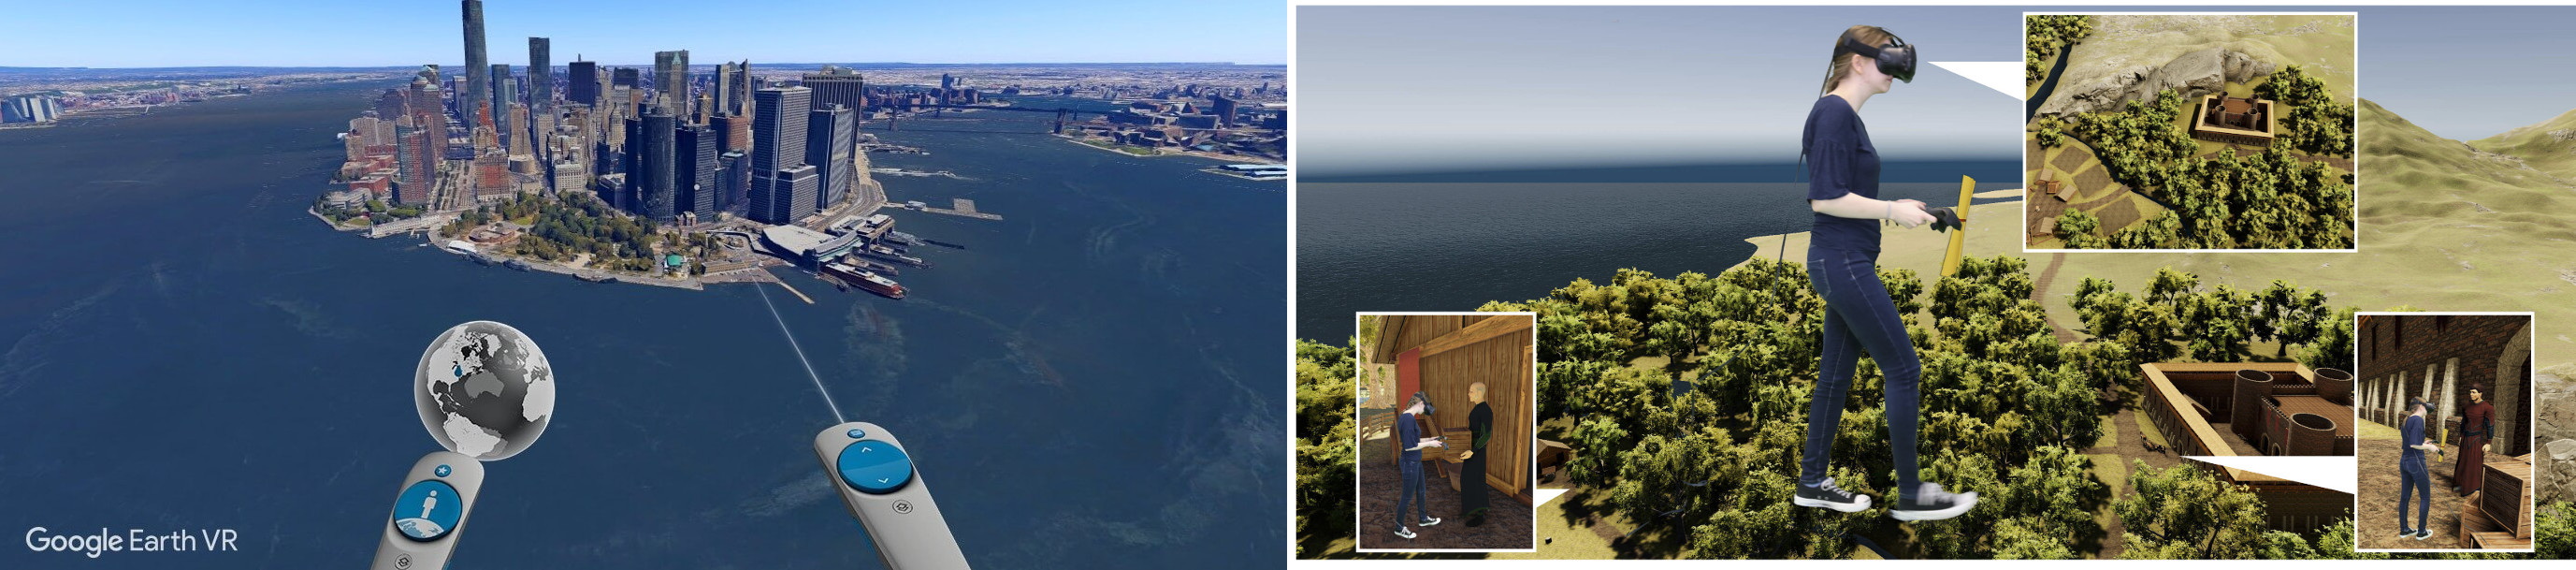
\includegraphics[width=\textwidth]{images/google_gulli.jpg}
  \caption{Google Earth VR (links) vereinigt \textit{Physical Movement}, \textit{Steering}, \textit{Manual Viewpoint Manipulation} und \textit{Physical Movement}, während GulliVR\cite{Krekhov2018GulliVR} dem Nutzer auf Riesengröße wachsen lässt, um große Distanzen zu überwinden}
  \label{fig:todo}
\end{figure}

In den letzten Jahren wurden zahlreiche Arbeiten zum Reisen in virtuellen Umgebungen entwickelt und veröffentlicht, die sich (zumeist) an den im letzten Kapitel beschriebenen Kriterien orientierten, wobei aber die Gewichtung dieser Qualtitätsmerkmale sehr varrierte, denn die zu bereisenden virtuellen Realitäten können verschiedenster Natur sein. Daher unterscheiden sich die Techniken zur Navigation anhand ihrer Motivation, der genutzten Hardware, der Nutzerzahl, aber nicht zuletzt auch der Umgebung.
In der akademischen Forschung sind die Umgebungen, für die eine entsprechende Navigation entwickelt werden, vielfältig.
Zum einen werden Techniken entwickelt, die sich primär für den Gebrauch im Freien eignen. Beispiele hierfür sind das Reisen zwischen mittelalterlichen Dörfern \cite{Krekhov2018GulliVR} oder in größerem Umfang die Navigation in hierarchisch strukturierten Umgebungen, bei denen der Nutzer wie bei Google Earth fließend zwischen Nachbarschaften, Städten, Ländern oder Kontinenten wechselt \cite{pierce_representations}.
Außerdem werden neben dem Manövrieren innerhalb von Gebäuden, wie Einkaufszentren oder einzelnen Stockwerken (z.B. \cite{Richardson1999SpatialEnvironments}, \cite{Liang2018EvaluatingEnvironments}) selbstverständlich auch Szenarien untersucht, bei denen es gilt sowohl Indoor als auch Outdoor zu navigieren, beispielsweise durch Haus und Terrasse einer Villa wie bei \cite{Dallat2018Giant}. 
Virtuelle Realitäten bieten aber auch die Möglichkeit sich durch Datensätze wie zum Beispiel der Visualisierung einer Punktwolke oder sich durch den menschlichen Körper \cite{Kopper2006DesignEnvironments} zu navigieren.

Durch die Möglichkeit beinahe alle vorstellbaren Szenarien in einer immersiven Umgebung darstellen zu können, sind die einhergehenden Motivationen zur Navigation vielfältig. Dennoch lassen sie sich in drei grundlegenden Typen klassifizieren: \textbf{Exploration}, \textbf{Search} und \textbf{Maneuvering} (\cite{Bowman2001AnDesign}, \cite{KulikBuildingTechniques}). 
Diese Einteilung lässt sich sowohl für Einzel- und Mehrbenutzernavigation, als auch für die Navigation auf gleichbleibenden oder unterschiedlichen Skalierungen vornehmen.
Exploration beschreibt dabei einen freien Navigationsvorgang, wie das Spazieren durch eine unbekannte Stadt. Dabei wird während des Bewegens die Umgebung erkundet, indem man sich umsieht, also eine Rotation des Standpunktes vornimmt. 
Dies kann man allerdings auch auf eine andere Skalierungsebene übertragen. Das entsprechende Beispiel wäre das freie Erkunden des Stadtplans, in dem man ohne sich eines Ziels bewusst zu sein, den Aufbau der Stadt ergründet. Klassischerweise tut man das in dem man die Lage wichtiger Punkte (z.B. Bahnhof, Stadtzentrum, Denkmäler etc.) zueinander betrachtet und mögliche Routen frei “inspiziert”.\\
Die Suche beschreibt dagegen den Vorgang des Findens des effizientesten Weges von einem Start A zu einem Ziel B. Auch hier lässt sich wieder das Navigieren in einer fremden Stadt als Beispiel nehmen. Befindet man in der “realen Skalierung” eines Touristen wäre die Orientierung an Wegweisern und Straßenschildern der Weg um die kürzeste Route von dem aktuellen Standpunkt zu einer Touristenattraktion. Hier kommt jedoch zumeist der Stadtplan ins Spiel, bei dem der Tourist eine bessere Übersicht hat und somit den effizienteren Weg schnell finden kann.\\
Während der Vorgang des Gehens in diesen Beispielen dem nach Bowman beschriebenen ”\textit{Travel}”-Prinzips entspricht, also der tatsächlichen Reise, während der Blick auf die Karte dem ”\textit{Wayfinding}” zuzuordnen ist. 
Im besten Fall kann eine Navigationstechnik all diese Ansprüche bedienen: Er kann sie nutzen, um den Weg zu finden und diesen schnell zu beschreiten, unabhängig ob er sein Ziel kennt oder einfach nur die ganze Umgebung ausgiebig erkunden will.

Das Manövrieren stellt eher das Verändern des Sichtpunkts um ein Objekt herum da, um es in verschiedenen Orientierungen zu betrachten oder um besser mit diesem interagieren zu können. Diese ist sehr viel feingliedriger und könnte im Beispiel des Touristen ein Umkreisen eines Denkmals sein, was dieser genauer betrachten will. Dieser Vorgang findet in den meisten Fällen (wie z.B. in unserer Multiuser Leinwand) durch das Bewegen des eigenen Körpers und des Kopfes statt und ist in diesem Fall kein Bestandteil einer Navigationstechnik.

Doch während beim Entwickeln einer neuen Technik die zu bereisende Umgebung und die Motivation, weshalb gereist wird, sicherlich wichtige Faktoren sind, stellt der wichtigste Gesichtspunkt die Art und Weise dar, in welcher navigiert wird. Bowman et al. \cite{Bowman2001AnDesign} unterteilen hierbei Navigation in 5 Metaphern: \textbf{Physical Movement}, \textbf{Manual Viewpoint Manipulation}, \textbf{Steering}, \textbf{Target-based Travel} und \textbf{Route Planning}. 
\textit{Physical Movement} beschreibt dabei, dass sich der oder die Nutzer in der realen Umgebung mit ihren (realen) Körpern bewegen. Dies kennt man von trackingbasierten Systemen wie der HTC Vive, bei denen sich der Nutzer mit seinem getrackten Headset in einem realen Umfeld bewegt und seine Bewegung in die virtuelle Umgebung, die dieser in diesem Moment sieht, umgesetzt wird.
Bei der \textit{Manual Viewpoint Manipulation} kann der Nutzer sich in der Welt ”entlanghangeln”. Dies geschieht, in dem er sich virtuellen Gegenständen oder ggf. in der Luft “festhält” und die virtuelle Welt zu sich “heranzieht”. 
In dreidimensionalen Computerspielen, wie z.B. Ego-Shootern oder Flugsimulatoren, findet man die vermutlich bekannteste Fortbewegungsweise, das \textit{Steering}. Hierbei kontrolliert der Nutzer zu jedem Zeitpunkt seine Translation und Rotation im Raum.
Gerade seit dem Aufkommen konsumentenfreundlicher Systeme der virtuellen Realität wird die Nutzung von \textit{Targed-based Travel} populärer: Hierbei spezifiziert der Nutzer sein Reiseziel und das System übernimmt die Transition zu diesem. 
Google Earth VR vereinigt dabei alle Metaphern bis auf \textit{Route Planning}. Durch das Anzeigen der Richtung mit dem Controller und gleichzeitigem Knopfdrücken kann man durch die Welt fliegen (\textit{Steering}). Alternativ kann man auch einen Punkt in der Welt greifen und zu sich heranziehen (\textit{Manual Viewpoint Manipulation}). Um einen \textit{Target-based Travel} einzuleiten, kann man auf der Weltkugel (vgl. Abbildung 8.1), welche man in der linken Hand hat, einen Punkt in der Welt selektieren und wird zu diesem teleportiert. Gleichzeitig ist es zu jedem Zeitpunkt möglich seine aktuelle Position durch Laufen im eigenen Trackingspace zu verändern (\textit{Physical Movement}) 

Ein bekanntes Beispiel dafür ist die in VR oft genutzte Teleportation, mit der der Nutzer sich über die Grenzen des Bereichs, den er durch physische Bewegung erreichen kann, hinfort bewegt (vgl. Abbildung 2.3).
Das \textit{Route Planning} stellt zu guter Letzt eine Technik da, mit der der Nutzer einen Weg spezifiziert, auf welchen ihn das System daraufhin bewegt. Dies erlaubt dem Nutzer während der Bewegung andere Aufgaben auszuführen und sich nicht ausschließlich auf die Reise zu konzentrieren. Die verwandten Arbeiten die im Folgenden vorgestellt werden, beziehen sich auf die Themen Gruppennavigation und Navigation über große Distanzen und nutzen diese Metaphern. Allerdings kann bereits an dieser Stelle verraten werden, dass \textit{Manual Viewpoint Manipulation} besonders aber \textit{Route Planning} nicht auftauchen, da sie nicht zu den populärsten Metaphern zählen.

\section{Navigation in Gruppen}
Bisher gibt es sehr wenige Arbeiten, die sich mit dem Thema der Gruppennavigation in virtuellen Umgebungen beschäftigen. Eine dieser Arbeiten, welche inhaltlich nahe am Thema dieser Arbeit ist, ist die Arbeit von Weißker et al. (\cite{WeisskerMulti-RayReality}). Darin wird eine neue Technik vorgestellt, die sich mit dem gemeinsamen Teleport von zwei Personen beschäftigt. Auch hier wird als beispielhaftes Szenario der Stadtführer, welcher einen zweiten Nutzer (passiver Nutzer, Passagier) durch eine Stadt führt, genannt. 
In diesem Fall spielt sich die Navigation allerdings im Vista-Raum ab und wird auf Head Mounted Display getestet. Sie stellt eine Erweiterung der oben genannten Teleporttechnik dar, wobei der passive Nutzer vom Führenden auf verschiedene Arten mitgenommen wird (\textit{Coupled, Vehicle und Congruent}. Die Technik in unserer Arbeit kann als Ergänzung zu dieser Arbeit gesehen werden. Dabei dient erstere für den Sprung über große Distanzen, letztere dann für kleinere Distanzen innerhalb des sichtbaren Bereichs. Einige Erkenntnisse gelten dabei für beide Distanzen: Zum einen ist es immens wichtig, dass der Navigator zu jedem Zeitpunkt die aktuellen Positionen seiner Mitreisenden kennt und auch weiß, wo diese Position nach dem Teleport sein werden um Kollision zu vermeiden und sicherzustellen, dass entsprechende POIs im Blickfeld von allen liegen. Dies gilt im Übrigen auch für die anderen Nutzer, damit sie sich auf die Konsequenzen des Sprungs einstellen können. Dieses wird dadurch ermöglicht, dass auch der passive Nutzer einen Strahl zu seinem voraussichtlichen Teleport Ziel angezeigt bekommt. Dies minimiert Fehler in der Platzierung durch den aktiven Nutzer und reduziert die kognitive Last beider Nutzer, führt allerdings zu einem etwas längeren Planungsvorgang vor der Reise. Weiterhin stellen die Autoren fest, dass das Wohlbefinden bzw. die Simulatorenkrankheit des passiven Nutzers nicht deutlich stärker ist, als bei einem Einzelnutzer Teleport. Verbunden mit der nötigen Aufmerksamkeit des aktiven Nutzers und einer effektiven Kommunikation wird somit eine erfolgreiche Navigation ermöglicht, sodass der passive Nutzer bei dieser nicht mit der Umgebung kollidiert. Dies stellt nämlich eine der größten Schwierigkeiten der gemeinsamen Navigation dar, womit sich Kulik et al. (\cite{Kulik2011C1x6}) beschäftigen. Diese befassen sich neben der Hardware unseres Lehrstuhls deren Weiterentwicklung acht Jahre später in dieser Arbeit genutzt wird mit dem Problem, dass nicht immer alle Gruppenmitglieder in einem gemeinsamen Tracking Space in den möglicherweise viel kleineren, virtuellen Raum passen. In diesem Fall wird allerdings die \textit{Steering} Navigation genutzt, von der sich jetzt schon abzeichnet, dass sie aufgrund der Dauer und des Motionflows für größere Distanzen weniger geeignet ist, als ein Teleportationsvorgang.
Ein weiterer Hinweis auf die Navigation mit mehreren Nutzern findet sich in der Arbeit von Beck et al.(\cite{BeckImmersiveTelepresence}). Hier bewegen sich zwei Gruppen gemeinsam in einer virtuellen Welt, wobei ihnen die Möglichkeit gegeben wird, sich unabhängig voneinander zu bewegen oder dem anderen Team zu folgen. Der besondere Aspekt dabei ist aber, dass sich die Nutzer in einer World in Miniature (siehe übernächster Absatz) sehen können und das andere Team in dieser selektieren und an einen anderen Ort bewegen können. Obwohl selbst die Autoren zugeben, dass diese Methode bei den Mitgliedern des Teams, welches versetzt wird, Unwohlsein auslöst, ist die Idee, eine WIM zur Navigation zu nutzen, indem man die Plattform der Nutzer in dieser platziert eine spannende und vielversprechende Vorgehensweise, auf die im übernächsten Absatz genauer eingegangen werden soll. 



\section{Skalierungsbasierte Techniken}
Viele Anwendungen und Programme bieten neben den allgemein genutzten sechs Freiheitsgraden, drei für Translation und drei für Rotation noch einen weiteren Freiheitsgrad:
Die fünf bekannten Metaphern (\textit{Steering} usw.) werden erweitert durch die Modifizierung der Größe des Nutzers in der virtuellen Umgebung. Dies hat zwei entscheidende Vorteile. Zum einen kann der Nutzer seine Umgebungen in verschiedenen Skalierungen betrachten. Ein Nutzer, der die Größe eines Riesen hat, kann eine Region weitaus besser Überblicken, während er in der Größe von wenigen Zenti- oder gar Millimetern kleinteilige Regionen einer Umgebung explorieren kann. Doch neben dem visuellen Vorteil bietet die Modifizierung der eigenen Größe einen für diese Arbeit viel wichtigeren Vorteil. In der Größe eines Riesen kann der Nutzer bei gleichbleibender wahrgenommener Geschwindigkeit viel größere Distanzen überwinden als in seiner normalen Größe mit normaler Laufgeschwindigkeit.
Dies machen sich zum Beispiel Krekhov et al. (\cite{Krekhov2018GulliVR}) in ihrer Arbeit zu nutze. Nach dem \textit{Physical Locomotion} Prinzip kann sich der Nutzer in einem realen Raum bewegen und dabei zwischen dem sogenannten \textit{Normal Mode} und \textit{Giant Mode} wechseln. Zweiteres bedeutet, dass der Nutzer auf die Größe eines “Giganten” vergrößert wird. Die Zielgröße wird dabei so festgelegt, dass der Nutzer das weiter entfernte Dorf, welches er zur Erfüllung seiner Aufgabe aufsuchen muss, erreichen kann, in dem er mit wenigen Schritten innerhalb seines realen Tracking Spaces zu diesem Dorf läuft, um sich dort wieder zu schrumpfen. In diesem \textit{Giant Mode} wird der Augenabstand so modifiziert, dass der Nutzer das Gefühl hat in einer Miniaturwelt zu stehen, anstatt über der Welt zu fliegen. Will der Nutzer sich wieder auf seine Ausgangsgröße zurück schrumpfen, bieten die Verfasser zwei Methoden: Beim \textit{Targeting} wird dem Nutzer mit einem Zielkreuz zu seinen Füßen angezeigt, wo er nach der Skalierung stehen wird, beim \textit{Pulling} wird der Nutzer, wenn er sich innerhalb eines festgelegten Areals befindet, während er geschrumpft wird zu einem vorher definierten Point of Interest bewegt, sodass er nach der Transition direkt vor diesem steht. (vgl. Abbildung)
Die drei Hypothesen, dass der Nutzer a) ein erhöhtes Präsenz-/ Überblicksgefühl hat, b) keine Cybersickness empfindet und c) signifikant mehr läuft, konnten in einer Vergleichsstudie, in der gegen die Fortbewegung durch das aus SteamVR bekannte Teleportieren getestet wurde, bestätigt werden.
Diese Ergebnisse lassen sich allerdings nur bedingt auf die Entwicklung einer Technik für mehrere Nutzer im kohärenten Workspace übertragen, da ein gemeinsames Laufen in einer Gruppe ein Problem darstellt. So müssten alle Nutzer gleichzeitig größer bzw. kleiner skaliert werden, damit die Kohärenz des Workspaces nicht aufgehoben wird. Zusätzlich muss dazu noch ein gemeinsames Laufen koordiniert werden, was nicht nur wegen der zumeist geringen Größe des Tracking Spaces ein schwieriges Unterfangen wäre. Denn in Hinblick auf die Nutzung an unserem semi-immersiven Leinwandsystem ist ein solcher gemeinsamer Spaziergang ausgeschlossen. Ansätze, wie sich der vorhandene Tracking Space wie z.B. durch ”\textit{Redirected Walking}” (\cite{RazzaqueRedirectedWalking}) besser nutzen lassen könnte, sind für mehrere Nutzer in gemeinsamen Workspaces und vorallem am Leinwandsystem ebenfalls keine Alternative. 
Dennoch lassen sich die Erkenntnisse zur schnelleren Überwindung von Distanzen und des erhöhten Präsenzgefühls durch den Blick von oben nutzen. Denkbar wäre z.B. ein gemeinsames Aufskalieren, mit anschließendem Teleportations- bzw. Steeringvorangs, wobei die wahrgenommene Reisedistanz deutlich abnimmt.

Einen ähnlichen Weg gehen McCrae et al.\cite{McCrae2009MultiscaleNavigation}.
Der Nutzer kann dabei also frei in der Welt umherfliegen, wobei seine Größe und seine Bewegungsgeschwindigkeits stets so modifiziert werden, dass er das Gefühl einer fließenden und gleichbleibenden Fortbewegungsgeschwindigkeit wahrnimmt. 
Die tatsächliche Größe und somit auch Geschwindigkeit, sowie die Anpassung der near- und far-clipping plane werden mit Hilfe einer sogenannten ”\textit{Cube Map}” bestimmt. Dabei wird ausgehend von der aktuellen Kameraposition in alle sechs kanonischen Richtungen ein 64x64 Bit Bild errechnet, welches die Distanzen zu allen Objekten kodiert (vgl. Abbildung). Anhand der minimalen Distanz dieser ”\textit{Cube Map}” werden die resultierenden Skalierungsparameter errechnet.
Das Resultat ist, dass Nutzer durch die Umgebung fliegen können ohne selbst manuelle Einstellungen der Skalierungsparameter ausführen zu müssen. Diese Vorgehensweise wird von Argelaguet et al. \cite{Dallat2018Giant} weiter verbessert, um Nutzern ein noch besseres Gefühl von konstanter Bewegungsgeschwindigkeit bei unterschiedlichen Skalierungen erhalten.
Kopper et al. \cite{Kopper2006DesignEnvironments} verfolgen den Ansatz, die Parameter entsprechend des jeweiligen Gebiets, in dem sich der Nutzer befindet, anzupassen. In ihrem Anwendungsfall wird der menschliche Körper und dessen Organe bereist. Die Auswahl der Parameter wird entsprechend des Volumens der \textit{Bounding Box} des Organs, in welchem man sich befindet, gewählt. Dabei bieten die Verfasser zwei Möglichkeiten zur Navigation: Zum einen können Nutzer wie in den zuvor genannten Arbeiten durch \textit{Steering} durch den Körper “fliegen”. Stoppen die Nutzer in einem Organ, so wird Augenabstand, Fluggeschwindigkeit und somit die wahrgenommene Körpergröße je nach vorherigen Parametern entweder verkleinert oder vergrößert. In der zweiten Möglichkeit, kann der Nutzer mit Hilfe einer Lupen Metapher Organe auswählen und wird dann automatisch in deren Zentrum gesetzt, wobei auch hier die Anpassung der Parameter stattfindet.
Der Ansatz der automatischen Anpassung der Navigations- und Stereoparametern wird so oder in abgewandelter Form auch bei Google Earth VR genutzt. Diese Technik kann und wird auch in Mehrbenutzerszenarien benutzt, jedoch benötigen \textit{Steering}-Techniken immer einen Steuermann. Dies wiederum bedeutet immer, dass es passive Nutzer gibt, die nicht an der Navigation und somit der Zielfindung beteiligt sind. Außerdem kommt es bei \textit{Steering}-Techniken in virtuellen Realitäten häufig zur \textit{Simulator Sickness} (vgl. \cite{Lackner2014MotionVomiting}).
Ein \textit{Targed-based}-Vorgehen wie in der zweiten Variante Koppers wäre für mehrere Anwender sicher besser geeignet, da sich hierbei die Nutzer vor der Reise über das Ziel einig werden können und gegebenenfalls auch so geplant werden kann, dass sich nach der Transition wirklich alle Nutzer innerhalb des gewünschten Organs bzw. allgemein Zielgebiets befinden können.

Generell lässt sich sagen, dass skalierungsbasierte Techniken einen guten Ansatz bieten, die bekannten Bewegungsmetaphern auf große Distanzen zu erweitern, dennoch lassen sich zahlreiche Kriterien aus Kapitel 2 mit den bisherigen Ansätzen nicht erfüllen:
\textit{Steering} und \textit{Physical Walking} wirken sich negativ auf die Bearbeitungszeit aus, der Nutzerkomfort für passive Nutzer wird ebenfalls eingeschränkt und auf das Prinzip der Gruppeninteraktion wird in keinem Ansatz eingegangen.

\section{Navigation mit Hilfe von World in Miniatures}

Ein weiterer Ansatz zur Navigation in virtuellen Umgebungen wurde bereits 1970 von Stoakley et al. \cite{Stoakley2010VirtualWIM} vorgestellt. Das Konzept der sogenannten \textit{World in Miniature} (im folgenden: WIM) beschreibt eine miniaturisierte Kopie der Umgebung bzw. Welt in der sich der Nutzer gerade befindet. Mit dieser Metapher ist es dem Nutzer nicht nur möglich einen exozentrischen Blick von oben auf die ihn umgebende Hauptszene zu werfen, sondern er kann diese Miniatur auch als Interface nutzen. Die Möglichkeiten dieses Interface sind dabei vielfältig. Genau wie in der Hauptszene bietet sie drei Möglichkeiten zur Interaktion: Selektion, Manipulation und Navigation.
Selektion und Manipulation bedeutet in diesem Zusammenhang, dass der Nutzer in die WIM “greifen” kann und dabei z.B. die Position und Ausrichtung eines Objektes verändern kann, wobei die Änderungen in der Miniaturwelt zeitgleich in der Hauptszene umgesetzt werden. Die Vorteile einer solchen Manipulation liegen (wortwörtlich) auf der Hand: Der Nutzer muss nicht mehr in der Hauptszene zu Objekten navigieren, sondern kann diese einfach in der WIM zu sich ziehen. 
Weiterhin besteht aber auch die Möglichkeit, dass der Nutzer die Repräsentation seiner selbst auswählt, um diese (und somit sich selbst) zum entsprechenden Objekt zu manövrieren. So wird die Metapher der Manipulation zur Navigationsmetapher.
Diese Metapher bedurfte allerdings weiterer Optimierung. Setzt man nämlich den Positionswechsel des Nutzers zeitgleich in der egozentrischen Sicht um, kann dies zu starker Desorientierung führen. In ihrer ursprünglichen Arbeit schlagen die Verfasser zwei Alternativen vor: Entweder wird der Navigationsvorgang erst nach dem Abschluss der Manipulation durchgeführt, in dem der Nutzer in seiner egozentrischen Sicht mit einem flüssigen Übergang an sein gewähltes Ziel animiert wird oder der Nutzer kann mehrere Manipulationen durchführen, welche erst zum Zeitpunkt eines Knopfdrucks umgesetzt werden (”\textit{batching}”). 
Diese beiden Vorschläge wurden von Stoakleys Kollegen Pausch et al. (\cite{5_pausch_WIM}) durch eine Option erweitert, in welcher der Nutzer, nachdem er seine Repräsentation platziert hat nicht in der Welt in Originalgröße zu diesem Ort animiert wird, sondern direkt in seine eigene Repräsentation in der WIM hinein, sodass er sich danach auch in dieser befindet.
Das hat den den entscheidenden Vorteil, dass der Nutzer seine Aufmerksamkeit nicht erst wieder auf die ihn umgebende Welt richten muss, sondern die Navigation in seinem aktuellen kognitiven Fokus stattfindet, was Verwirrung und Desorientierung mindert. In diesem Fall wird die vormals exozentrische zur egozentrischen Ansicht.
Die Autoren geben allerdings zu Bedenken, dass bei diesem ”Zoom-In” Vorgang Kollisionen mit der Umgebung stattfinden können, welche durch vorherige Routenplanung ausgeschlossen werden müssten und dass die zurück zu legenden Distanzen die bei dieser Transition sehr groß sein können. 
Neben dem - in dieser Technik vorhandenen - Motionflow, der bei der Entwicklung unserer Technik ausgeschlossen werden soll, um Unwohlsein zu minimieren, spricht besonders der erste der genannten Aspekte gegen eine Nutzung dieser Technik für mehrere Nutzer. Denn während sich bei einer Gruppe von Nutzern eine solche Transition wegen der verschiedenen Standpunkte sowieso schon schwerer gestaltet, muss zusätzlich Rücksicht auf eventuelle Kollisionen genommen werden.

Eine weitere Möglichkeit, eine WIM zur Navigation zu benutzen, wurde im Anschluss auf die Arbeit von Staokley von LaViola et al. (\cite{LaViola2004Hands-freeEnvironments}) in Form der sogenannten  ”\textit{Step WIM}”  vorgestellt.
Eine zentrale Motivation dieser Arbeit war, die WIM - anders als bei Stoakley - nicht in der Hand halten zu müssen und die Hände somit für andere Aktivitäten nutzen zu können. 
Um dieses Kriterium einzuhalten wird die WIM auf den Boden, der sich im Zentrum von drei würfelförmig angeordneten 3D Leinwänden befindet, projiziert (vgl. Abbildung). Das hat weiterhin zum Vorteil, dass die WIM nicht mehr im Sichtfeld ist und somit keine wichtigen Teile der Szene verdeckt. 
Um eine Interaktion mit der Projektion zu ermöglichen, entwickeln die Autoren eine Vielzahl an Techniken, in denen unter anderem das Tracking der Hüfte sowie sogenannte ”\textit{Interaction Slippers}”, also Schuhe, welche als Eingabegerät dienen, genutzt werden.
So kann der Nutzer innerhalb der WIM zum gewünschten Ziel laufen und ohne die Nutzung seiner Hände den Befehl geben, dass die WIM an der Stelle an welcher er sich befindet hochskaliert wird, sodass der Nutzer sich an tatsächlich an der gewünschten Stelle befindet.
Auch kann der Nutzer die WIM durch Laufen skalieren. Die vorgestellten Interaktionstechniken bringen allerdings einen nicht zu unterschätzenden kognitiven Aufwand mit sich. 
Um die Navigation einzuleiten muss der Nutzer z.B. seine Zehen zusammenführen oder mit der Hüfte eine Hüpfbewegung machen. Der Skalierungsprozess wiederum wird durch das Zusammenführen der Fersen initiiert, woraufhin die WIM durch Laufen skaliert wird und das Zentrum der Skalierung durch die Kopfposition des Nutzers bestimmt wird, bis dieser wieder seine Fersen zusammenführt. Gleichzeitig kann der Nutzer die WIM oder sich selbst in der Welt translatieren, wobei hier die Blickrichtung (in Richtung Boden oder Wand) entscheidet, welche der beiden Funktionen ausgeführt wird.
Auch wenn diese Interaktionen (vor allem das Skalieren der WIM) ein wichtiger Teil des Navigationsprozesses sind, stellt sich die Frage, ob der Interaktionsfluss nicht doch durch die ungewohnte Nutzung der Füße und Hüfte als Eingabegerät eingeschränkt wird.
Im Hinblick auf die Benutzung durch mehrere Nutzer lässt sich sagen, dass durch die gute Sichtbarkeit der Bodenprojektion alle Nutzer eine gute Vorstellung ihrer aktuellen Position und der Interaktion mit der WIM hätten. Eine Umsetzung dieser Technik, bei der ein geübter Navigator eine Personengruppe mit Hilfe der Step WIM durch eine virtuelle Umgebung leitet ist durchaus denkbar. Dabei wäre denkbar die, doch etwas ungewohnten Fußeingaben, durch Eingaben mit einem Eingabegerät in der Hand zu ersetzen. So könnte man bei den Pointern, wie sie in unserem System genutzt werden, durch ihren aktuellen Winkel den Kontext ableiten: Neigt man den Controller soweit nach unten, dass sein Vorwärtsvektor nicht mehr die Leinwand, sondern den Boden schneidet, würde automatisch die Interaktion mit der WIM, statt mit der Szene, aktiviert.

Während LaViola et al. ihre ”\textit{Step WIM}” auf kontinuierliche Weise auf- und wieder abskalieren, um weiter entfernte Regionen zu erreichen, nutzen Pierce et al. \cite{pierce_representations} eine diskrete Anzahl von hierarchisch strukturierten Voransichten. Dabei liegt der Schwerpunkt darauf große, virtuelle Umgebungen sehr schnell zu bereisen.
Mit dem Grundgedanken, dass sich Nutzer vor allem mit Hilfe von visuellen Orientierungspunkten, wie Denkmälern, Sehenswürdigkeiten oder sonstigen eindrücklichen Objekten in einer Umgebung zurechtfinden, stellen die Verfasser dem Nutzer Repräsentationen von Orten zur Verfügung, die er nutzen kann, um an diese Orte zu reisen.
Dabei kann jede Repräsentation als eine Art WIM angesehen werden, wobei diese hierarchische Skalierungslevel der Umgebung darstellen. In der niedrigsten Hierarchiestufe sind diese Repräsentationen tatsächliche Kopien der dargestellten Welt. In allen Stufen darüber zeigen die Repräsentationen vereinfachte Darstellungen des Gebiets, indem nur für die Identifizierung dieses Gebiets wichtige Orientierungspunkte zu sehen sind (vgl. Abbildung).
Die Hierarchien entsprechen dabei den im Alltag benutzten Begriffen “Nachbarschaft”, “Stadtteil”, “Stadt”, “Region”, “Land”, “Bundesland”, und so weiter.
Will der Nutzer nun von einer Stadt in eine andere reisen, z.B. von Lyon nach Paris, kann er sich durch die Hierarchie des Baumes navigieren. Die Repräsentationen des aktuellen Levels, so wie dem Level darüber werden um den Nutzer herum angezeigt. Deutet er auf sie und bestätigt dies mit einem Knopfdruck, wird die gewählte Repräsentation in seine Hand befördert. Handelt es sich um eine vereinfachte Repräsentation, also nicht auf dem niedrigsten Level, kann er aus dieser die gewünschte Repräsentation des nächst- niedrigeren Levels herausziehen. 
Gehört die Repräsentation zum untersten Level (also zur “Nachbarschaft”), kann der Nutzer sie in seiner Hand so positionieren, dass er aus dem gewünschten Blickpunkt in die tatsächliche WIM schaut. Bestätigt er diesen, berechnet das System den korrespondierenden Sichtpunkt in der Hauptszene und der Nutzer wird automatisch an diesen Punkt teleportiert.
Diese Vorgehensweise bietet mehrere Vorteile: Zum einen ist eine schnellere und effizientere Vorgehensweise als die Traversion eines Baumes zum Erreichen entfernter Orte kaum möglich. Zum anderen stellt die finale Positionsauswahl durch Ausrichtung der WIM und Berechnung des korrespondierenden Blickpunkts eine intuitive Möglichkeit zur Zielbestimmung des Teleports. Diese Vorgehensweise kann allerdings schlecht in Mehrbenutzerszenarien angewandt werden, da immer nur eine Person in der Lage ist, den Blickpunkt in der WIM zu bestimmen. Die anderen wissen infolgedessen nicht zwangsläufig, welche Position dieser Nutzer ausgewählt hat.

Ein Lösungsansatz für diese Problematik lässt sich in der Arbeit von Kunert et al. (\cite{Kunert2014Photoportals}) finden.
Mit dem sogenannten Photoportal stellen die Verfasser ein Werkzeug vor, mit dem es möglich ist, zwei- und dreidimensionale “Fotos” in einer virtuellen Umgebung aufzunehmen.
Diese Fotos können, in einer Galerie gespeichert, von anderen Nutzern aufgerufen und betrachtet werden. Da diese Fotos auch in Form von dreidimensionalen Würfeln dargestellt werden können (vgl. Abbildung), kann man diese als WIMs betrachten.
Im Gegensatz zu den bisher vorgestellten WIMs können diese allerdings auch unterschiedlich skalierte Ausschnitte einer Szene repräsentieren. Wie in der ersten Abbildung zu erkennen ist, kann eine solche WIM wie in diesem Beispiel eine ganze Burg umfassen, aber auch nur den Ausschnitt eines Stockwerks, wie in der zweiten Abbildung. Durch Skalierung der Szene innerhalb der Portalbox kann der Nutzer dabei bestimmen, was genau er sehen will.
Da diese Fotos nichts anderes als Referenzen zu anderen Orten darstellen, können diese auch als Portaleingang zu diesen Orten genutzt werden.
Für einen einzelnen Nutzer bietet das System die Möglichkeit, dass er seinen Kopf in das Foto “hineinsteckt”, welches in etwa mit der Festlegung des Blickpunktes bei Pierce et al. aus dem letzten Abschnitt vergleichbar ist. In diesem Fall wählt der User nicht erst einen Blickpunkt, woraufhin das System den Teleport einleitet, sondern der Nutzer wird nahtlos von der Hauptszene in die vorher festgelegte (WIM-)Ansicht transferiert. Da aber die Photoportal Technik auf Mehrbenutzer hin entwickelt ist, kann der Einzelnutzer mit dieser Methode keinen Ortswechsel für alle Nutzer einleiten. Stattdessen gibt das System die Möglichkeit in einen für alle sichtbaren Galeriemodus zu wechseln. Dabei werden alle bisher aufgenommenen Fotos so positioniert, dass alle Nutzer diese sehen können. Will man eine Transition aller Gruppenmitglieder zu einem der aufgenommenen Orte unternehmen, so kann man ein Foto selektieren. Die Aufnahme fungiert in diesem Fall als “Guckloch” in die neue Szene und vergrößert sich daraufhin, bis der komplette Sichtbereich aller Nutzer gefüllt ist. In diesem Moment ist der Übergang vollzogen und die Nutzer befinden sich tatsächlich an dem vorher ausgewählten Ort. 
Auf diese Art und Weise wird ein Teleport ohne jeglichen Motionflow durchgeführt, der dennoch nicht abrupt und für alle Nutzer nachvollziehbar ist.
Die vorgestellte Technik bietet allerdings bisher keine Möglichkeit diese Fotos beziehungsweise Portaleingänge zu erstellen, ohne dass jemand vorher bereits an diesem Ort war und eine Aufnahme erstellt hat. Weiterhin wissen zwar alle Nutzer bereits vor Antritt der Reise, wie der Ort, an welchen sie reisen werden, aussieht, jedoch nicht zwangsläufig, wo sich dieser befindet.
Dies beides sind Faktoren, die es bei der Entwicklung einer reinen Navigationstechnik berücksichtigt werden müssen, wobei die zahlreichen anderen Funktionen der Photoportale für eine solche Technik nicht zwangsläufig gebraucht werden und auf Grunde ihrer Vielzahl einer schnellen und effektiven Navigation eher im Weg stehen.

Die Auseinandersetzung mit den verschiedenen Möglichkeiten zur Reise über große Distanzen legt bereits nahe, dass der Ansatz WIMs zu nutzen wohl der attraktivste ist:
Richtig platziert, können alle Nutzer die WIM überblicken und in dieser da Ziel ihrer Reise wählen. Sie bietet somit Raum, die Navigation mit allen Gruppenmitgliedern zu planen. Schon Stoakley et al. zeigten, wie schnell Nutzer dieses Interface für alle mögliche Interaktionen nutzen, ohne dass sie von der genutzten Metapher abgelenkt werden und dabei ein kognitives Abbild der Umgebung erstellen. 
Letzteres ist ein Aspekt, der große Vorteile im Hinblick auf die Raumwahrnehmung bietet, die im nächsten Kapitel weiter untersucht werden soll.
